\section{Results and Conclusions}

After testing every dataset on each of our models, we are able to observe a number of trends. In classification datasets, there is a distinct difference in classification accuracy between feed-forward and RBF networks. All three of our classification datasets showed greater performance when classified using an RBF network. Additionally, the prediction accuracy of feed-forward models consistently decreased as the number of hidden layers increased (Figure 4.1).

In regression datasets, the addition of hidden layers seems to result in reduced error in feed-forward networks, as networks with one hidden layer displayed lower mean actual error for every regression dataset tested when compared to the results of the same validation and training set on a feed-forward network with no hidden layers, though error appears to increase again when networks have two hidden layers (Figure 4.2).

Although the performance changes which result from additional hidden layers appear to vary based on whether the dataset tested was a classification or regression set, the highest performance was seen unanimously in one of the RBF models in every experiment.

\begin{figure}[b]
	\centering
	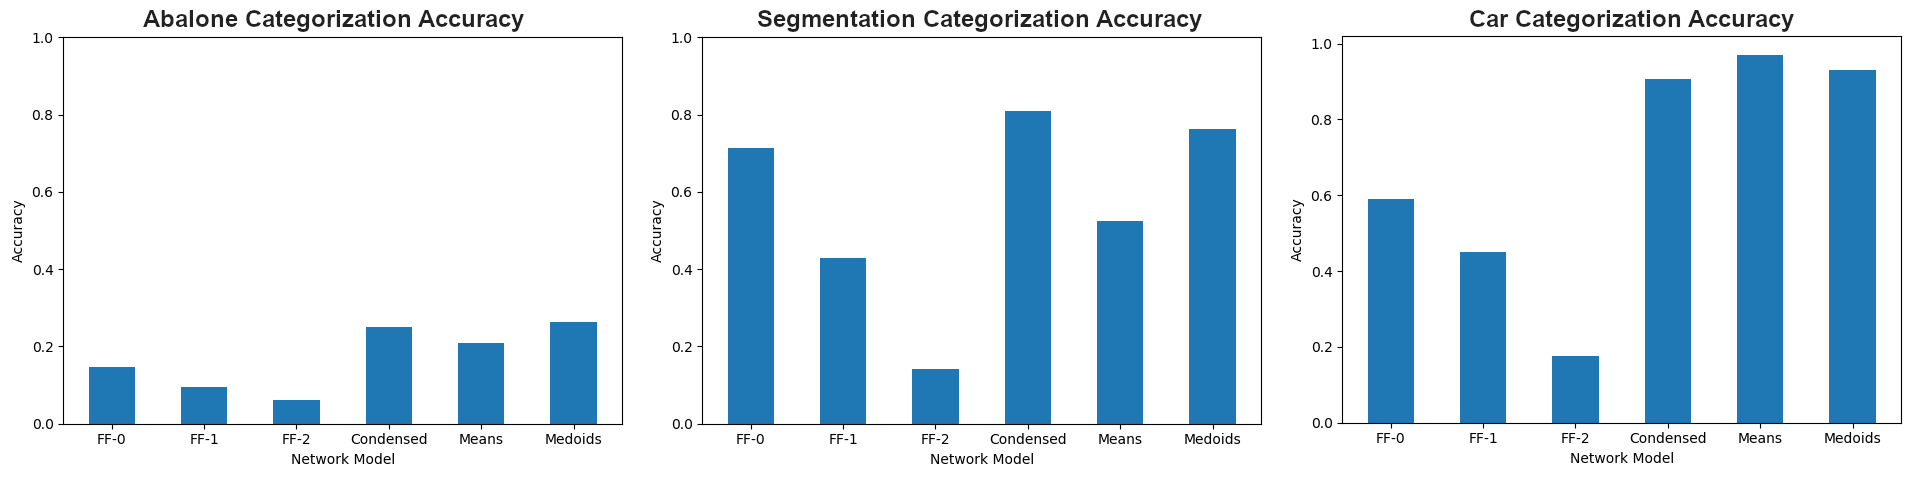
\includegraphics[width=\linewidth]{images/classification_results.png}
	\caption{Accuracy for each model applied to each regression dataset.}
\end{figure}

\begin{figure}[t]
	\centering
	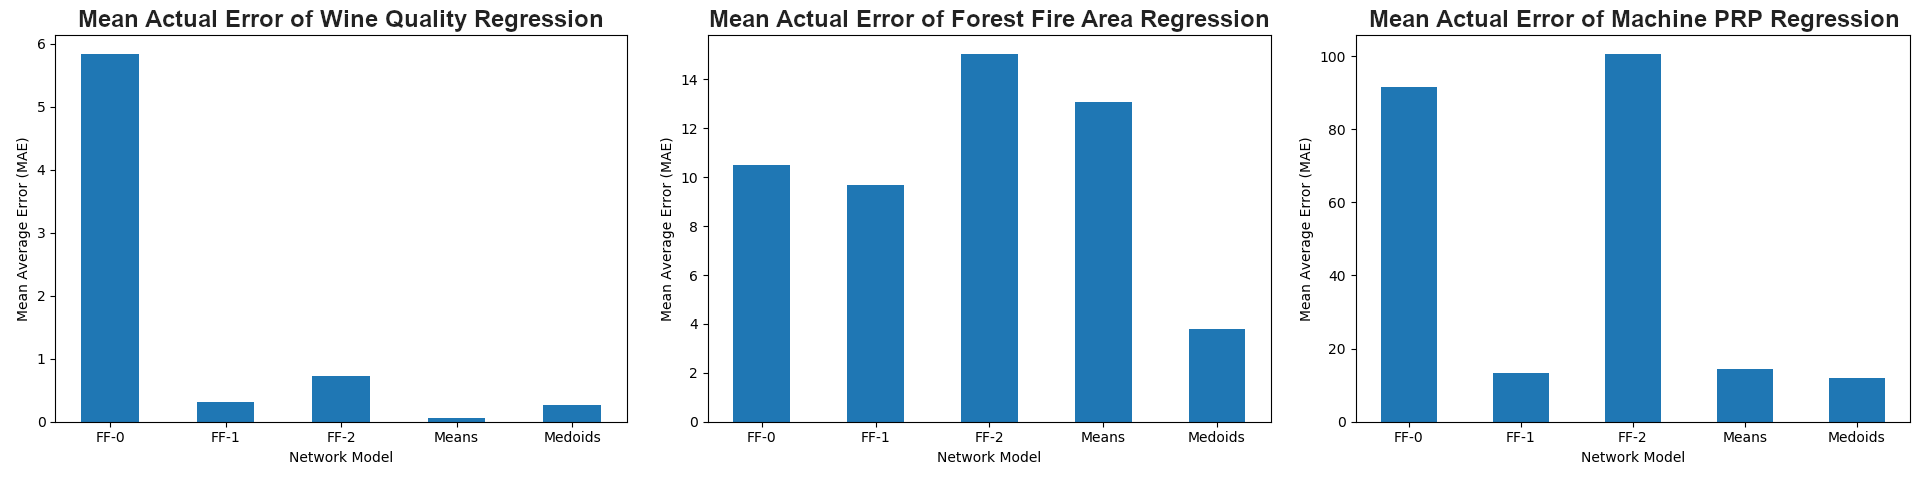
\includegraphics[width=\linewidth]{images/regression_results.png}
	\caption{Mean actual error for each model applied to each regression dataset.}
\end{figure}

\pagebreak

\begin{table}[t]
	\begin{tabularx}{\linewidth}{|c|X|X|X|X|X|X|}
		\hline
		Dataset & \textit{Abalone} & \textit{Car} & \textit{Segment.} & \textit{Machine} & \textit{Wine Quality} & \textit{Forest Fires} \\
		\hline
		$z$ Statistic & 27.392 & 8.587 & 6.228 & 0.0311 & 25.177 & 19.601 \\
		\hline
		$p$ Value & $<$ 0.00001 & $<$ 0.00001 & $<$ 0.00001 & 0.48759 & $<$ 0.00001 & $<$ 0.00001 \\
		\hline
	\end{tabularx}
	\caption{$z$ statistics and corresponding $p$ values for the difference in performance observed from the highest performing feed-forward and radial basis function variations in each dataset.}
\end{table}

In order to generally compare the feed-forward and radial basis function models for each dataset, we performed significance calculations on the highest performing variant for both models (Table 4.1). For all datasets but the \textit{machine} set, we are able to observe that the difference in performance was statistically significant within a confidence interval of 99.99\%. The difference in performance observed in the machine dataset can not be considered statistically significant within any reasonable confidence interval ($<$ .10).

From the results of our significance calculations, we are able to conclude that the performance of our radial basis function network was superior to the performance of our feed-forward network for the \textit{abalone}, \textit{car}, \textit{segmentation}, \textit{wine quality}, and \textit{forest fires} datasets. 


